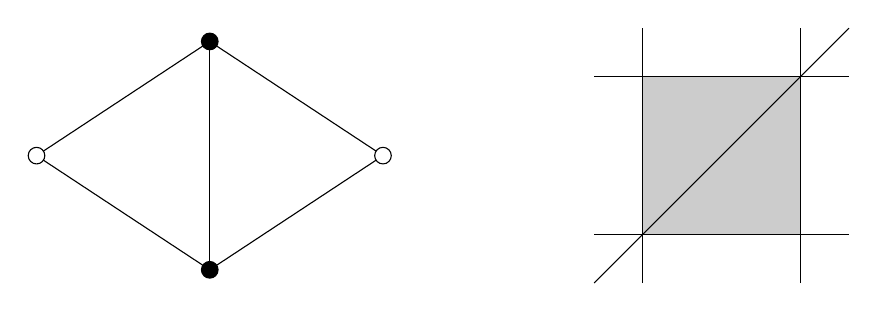
\begin{tikzpicture}[xscale=1,yscale=1]
\coordinate (a) at (-2.2,0);
\coordinate (b) at (0,1.45);
\coordinate (c) at (0,-1.45);
\coordinate (d) at (2.2,0);
\draw (a) -- (b) -- (d) -- (c) -- (a);
\draw (b) -- (c);
\draw[fill=white] (a) circle (3pt);
\draw[fill=black] (b) circle (3pt);
\draw[fill=black] (c) circle (3pt);
\draw[fill=white] (d) circle (3pt);

\def\a{6.5}
\draw[fill=black!20] ({-1+\a},-1) -- ({\a+1},-1) -- ({\a+1},1) -- ({\a-1},1) -- cycle;
\draw ({\a-1},-1.618) -- ({\a-1},1.618);
\draw ({\a+1},-1.618) -- ({\a+1},1.618);
\draw ({\a-1.618},-1) -- ({\a+1.618},-1);
\draw ({\a-1.618},1) -- ({\a+1.618},1);
\draw ({\a-1.618},-1.618) -- ({\a+1.618},1.618);
\end{tikzpicture}